\documentclass{article}
\usepackage[final]{nips_2017}
\usepackage{polski}
\usepackage[utf8]{inputenc}    % allow utf-8 input
\usepackage[T1]{fontenc}       % use 8-bit T1 fonts
\usepackage{hyperref}          % hyperlinks
\usepackage{url}               % simple URL typesetting
\usepackage{booktabs}          % professional-quality tables
\usepackage{amsfonts}          % blackboard math symbols
\usepackage{nicefrac}          % compact symbols for 1/2, etc.
\usepackage{microtype}         % microtypography
\usepackage[section]{placeins} % figures kept in sections
\usepackage{graphicx}          % images
\graphicspath{ {./img/} }
\usepackage{multirow}
\usepackage{float}             % figures in place
\usepackage{caption}		   % smaller margin after figure

\renewcommand{\figurename}{Wykres}
\setlength{\belowcaptionskip}{-20pt}

\title{  Regularyzacja\\Sieci Neuronowe 2020 }

\author{
  Jakub Ciszek \\
  238035\\
}

\begin{document}

\maketitle

\newpage
\tableofcontents
\newpage

Cały kod wykorzystany w zadaniu znajduje się pod adresem: \url{https://github.com/Greenpp/sieci-neuronowe-pwr-2020}

\section{Opis badań}
\subsection{Plan eksperymentów}

Wszystkie eksperymenty zostały przeprowadzone 10 razy. Losowość przy inicjalizacji wag oraz generacji danych nie została narzucona żadnym ziarnem. Podczas badań przyjęto górną granicę 40 epok, po przekroczeniu której, uczenie zostawało przerywane. Ze względu na charakter zadania (klasyfikacja) na ostatniej warstwie użyto funkcji Softmax, a za funkcję straty przyjęto Entropię krzyżową. Przyjęto następującą architekturę sieci: 784, 512, 256, 128, 10; za funkcję aktywacyjną posłużyła ReLU, wagi zostały wylosowane z przedziału \($-0.1 -- 0.1$\)
Z powodów wydajnościowych testowanie modelu przeprowadzano co każde 1024 przykłady.\\
Zostały przeprowadzone następujące badania:
\begin{itemize}
	\item Wpływ dropoutu na przebieg procesu uczenia.
	\item Wpływ regularyzacji L1 na przebieg procesu uczenia.
	\item Wpływ regularyzacji L2 na przebieg procesu uczenia.
	\item Wpływ regularyzacji L1,L2 na przebieg procesu uczenia.
\end{itemize}
Podczas wizualizacji funkcji straty pominięto pierwsze 10 pomiarów dla lepszej czytelności.

\subsection{Charakterystyka zbiorów danych}

Danymi użytymi w zadaniu jest zbiór ręcznie pisanych cyfr \(0-9\) - MNIST. Na zbiór składa się 70,000 obrazów wielkości 28x28 pikseli, co po przekształceniu odpowiadało 784 elementowemu wektorowi wejściowemu i 10 klasom na wyjściu. Użyta w zadaniu wersja została podzielona na 3 zbiory:
\begin{itemize}
	\item Uczący - 50,000 przykładów.
	\item Walidujący - 10,000 przykładów.
	\item Testowy - 10,000 przykładów.
\end{itemize}
W trakcie eksperymentów wykorzystano jedynie pierwsze 10,000 przykładów zbioru uczącego i testowy. Zbiór uczący został ograniczony aby łatwiej pokazać wpływ regularyzacji na przeuczenie.

\newpage
\section{Eksperymenty}

\subsection{Wpływ dropoutu na przebieg procesu uczenia}
\subsubsection*{Założenia}
\begin{table}[H]
	\caption{Stałe dla eksperymentu 1}
	\label{tabela-const-1}
	\centering
	\begin{tabular}{lr}
		\toprule
		Parametr      & Wartość \\
		\midrule
		Regularyzacja & Dropout   \\
		\bottomrule
	\end{tabular}
\end{table}

Zmienną w tym eksperymencie była szansa na wyłączenie połączenia. Prawdopodobieństwo przyjmowało wartości ze zbioru \(\{$0.0, 0.2, 0.5, 0.8$\}\)
\subsubsection*{Przebieg}

Warstwy dropout zostały ustawione po wszystkich warstwach oprócz ostatniej, wszystkie przyjmowały taką samą szanse na wyłączenie połączenia. Podczas eksperymentu model został zainicjalizowany 10 razy dla każdej z badanych wartości oraz wyuczony, uzyskane wyniki zostały zapisane w postaci pliku .plk do dalszej analizy.

\subsubsection*{Wyniki}
\begin{figure}[H]
	\centering
	\caption{TODO}
	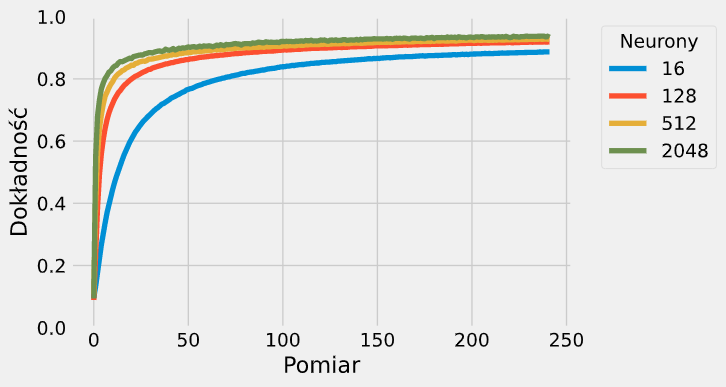
\includegraphics[width=\textwidth]{hidden_acc.png}
	\label{fig:res11}
\end{figure}

\begin{table}[H]
	\caption{TODO}
	\label{tabela-res-11}
	\centering
	\begin{tabular}{rrr}
		\toprule
		Prawdopodobieństwo & Dokładność [\%] \\
		\midrule
		0.0                 & --                 \\
		0.2                 & --                 \\
		0.5                 & --                 \\
		0.8                 & --                 \\
		\bottomrule
	\end{tabular}
\end{table}

\subsubsection*{Wnioski}

TODO
\newpage
\subsection{Wpływ regularyzacji L1 na przebieg procesu uczenia}
\subsubsection*{Założenia}
\begin{table}[H]
	\caption{Stałe dla eksperymentu 2}
	\label{tabela-const-2}
	\centering
	\begin{tabular}{lr}
		\toprule
		Parametr      & Wartość \\
		\midrule
		Regularyzacja & L1        \\
		Lambda        & 0.05      \\
		\bottomrule
	\end{tabular}
\end{table}

\subsubsection*{Przebieg}

Podczas eksperymentu model został zainicjalizowany 10 razy dla każdej z badanych wartości oraz wyuczony, uzyskane wyniki zostały zapisane w postaci pliku .plk do dalszej analizy.

\subsubsection*{Wyniki}
\begin{figure}[H]
	\centering
	\caption{TODO}
	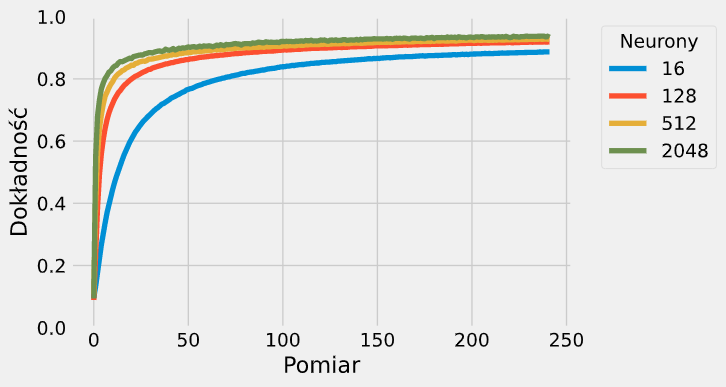
\includegraphics[width=\textwidth]{hidden_acc.png}
	\label{fig:res21}
\end{figure}

\subsubsection*{Wnioski}

TODO

\newpage
\subsection{Wpływ regularyzacji L2 na przebieg procesu uczenia}
\subsubsection*{Założenia}
\begin{table}[H]
	\caption{Stałe dla eksperymentu 3}
	\label{tabela-const-3}
	\centering
	\begin{tabular}{lr}
		\toprule
		Parametr      & Wartość \\
		\midrule
		Regularyzacja & L2        \\
		Lambda        & 0.05      \\
		\bottomrule
	\end{tabular}
\end{table}

\subsubsection*{Przebieg}

Podczas eksperymentu model został zainicjalizowany 10 razy dla każdej z badanych wartości oraz wyuczony, uzyskane wyniki zostały zapisane w postaci pliku .plk do dalszej analizy.

\subsubsection*{Wyniki}
\begin{figure}[H]
	\centering
	\caption{TODO}
	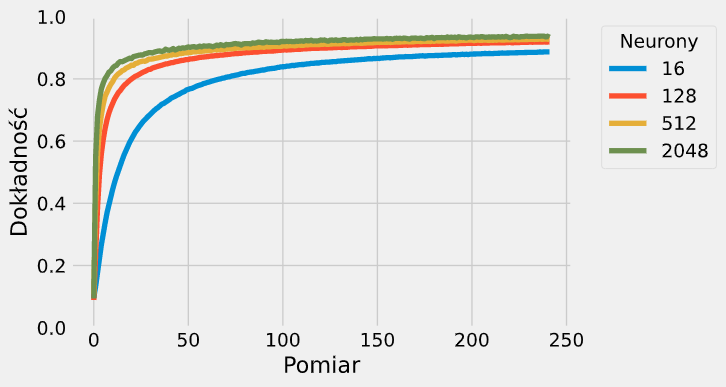
\includegraphics[width=\textwidth]{hidden_acc.png}
	\label{fig:res31}
\end{figure}


\subsubsection*{Wnioski}

TODO

\newpage
\subsection{Wpływ regularyzacji L1,L2 na przebieg procesu uczenia}
\subsubsection*{Założenia}
\begin{table}[H]
	\caption{Stałe dla eksperymentu 4}
	\label{tabela-const-4}
	\centering
	\begin{tabular}{lr}
		\toprule
		Parametr      & Wartość \\
		\midrule
		Regularyzacja & L1,L2     \\
		Lambda1       & 0.025     \\
		Lambda2       & 0.025     \\
		\bottomrule
	\end{tabular}
\end{table}

\subsubsection*{Przebieg}

Podczas eksperymentu model został zainicjalizowany 10 razy dla każdej z badanych wartości oraz wyuczony, uzyskane wyniki zostały zapisane w postaci pliku .plk do dalszej analizy.

\subsubsection*{Wyniki}
\begin{figure}[H]
	\centering
	\caption{TODO}
	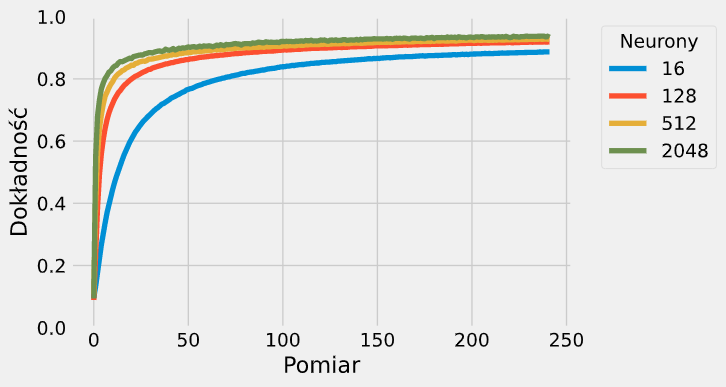
\includegraphics[width=\textwidth]{hidden_acc.png}
	\label{fig:res41}
\end{figure}

\subsubsection*{Wnioski}

TODO


\newpage
\section{Wnioski}

\begin{itemize}
	\item TODO
\end{itemize}

\end{document}